%Texlive-full Version 3.141592-1.40.3 (Web2C 7.5.6)
%TexStudio Version 2.7.0

%\documentclass[answers]{exam}
\documentclass{exam}% choose this one to have questions only

\usepackage[utf8]{inputenc}
\usepackage{graphicx}
\usepackage{subcaption}

\usepackage{lmodern}
\usepackage[a4paper]{geometry}

\usepackage{hyperref}
\usepackage{enumitem}
% \usepackage{nomencl}\makenomenclature

\usepackage{graphicx}
\usepackage{amsmath}
\usepackage{amssymb}
\usepackage{amsthm}

\usepackage{pstricks}
\usepackage{pst-node}
\usepackage{color}
\usepackage[ddmmyyyy]{datetime} 

\usepackage{listings}
%\lstset{language=C++,basicstyle=\scriptsize \color{green},identifierstyle=\color{orange},keywordstyle=[1]\color{blue},columns=fullflexible}
\lstset{language=C++,basicstyle=\scriptsize, keywordstyle=\color{blue}, stringstyle=\color{black},	commentstyle=\color{black} }


\begin{document}
\begin{titlepage}
%%%%%%%%%%%%%%%%%%%%%%%%%%  LOGO  %%%%%%%%%%%%%%%%%%%%%%%%%%%%%%%%%%%%%%%%%
\begin{center}
\begin{pspicture}(-7,0)(7,2)
%\psline(-7,0)(7,2)
\rput(-3.5,3){\href{http://ancoa.com/}{
\includegraphics[scale=0.3]{Ancoa_Logo}}}
\end{pspicture}
\end{center}

%%%%%%%%%%%%%%%%%% DOCUMENT TITLE %%%%%%%%%%%%%%%%%%%%%%%%%
\vspace{1cm}

\begin{center}
\resizebox{14cm}{0.8cm}{Test Mini Analytics}
\end{center}
%%%%%%%%%%%%%%%%%% DOCUMENT TITLE %%%%%%%%%%%%%%%%%%%%%%%%%
\begin{center}
Version : \today
\end{center}
\vspace{2cm}
\paragraph{}
This is a test for a junior analytics developer. The recommended time for the test would be 3h, but the candidate is free to spend time on the test. It is desirable to give us the time you've spend to do the test. Please send the result as a zip file to :
{\renewcommand\labelitemi{}
\begin{itemize}
	\item andrew.louth@ancoa.com
	\item simon.vella@ancoa.com
	\item chithanh.nguyen@ancoa.com
\end{itemize}
}

%%%%%%%%%%%%%%%%%% ABSTRACT %%%%%%%%%%%%%%%%%%%%%%%%%
\vfill
\begin{center}
Ancoa Software Ltd \copyright \hbox{ }2017.
\end{center}
\end{titlepage}
% % % % % % % % % % % % % % % % % % % % % % % % % % % % % % % % % % % % % % %
\newpage
%%%%%%%%%%%%%%%%%%%%%%%%%%%%%%%%%%%%%%%%%%%%%%%%%%%%%%%%%%%%%%%%%%%%%%%%%%%%%%%%%%%%%%%%%%
%%%%%%%%%%%%%%%%%%%%%%%%%%%%%%%%%%%%%%%%%%%%%%%%%%%%%%%%%%%%%%%%%%%%%%%%%%%%%%%%%%%%%%%%%%
\paragraph{General idea of the program}
The program has two components : the data feeder in real time, and a analytics API that process the data in real time, analyse and trigger a warning message if it found appropriate. Since the real data feeder could be complicated, we use a 'fake' data feeder. It load the whole offline data from a csv file, then give out one by one element. The Analytics take the data element one by one given by the system, and process it.

\begin{figure}[h]
\centering
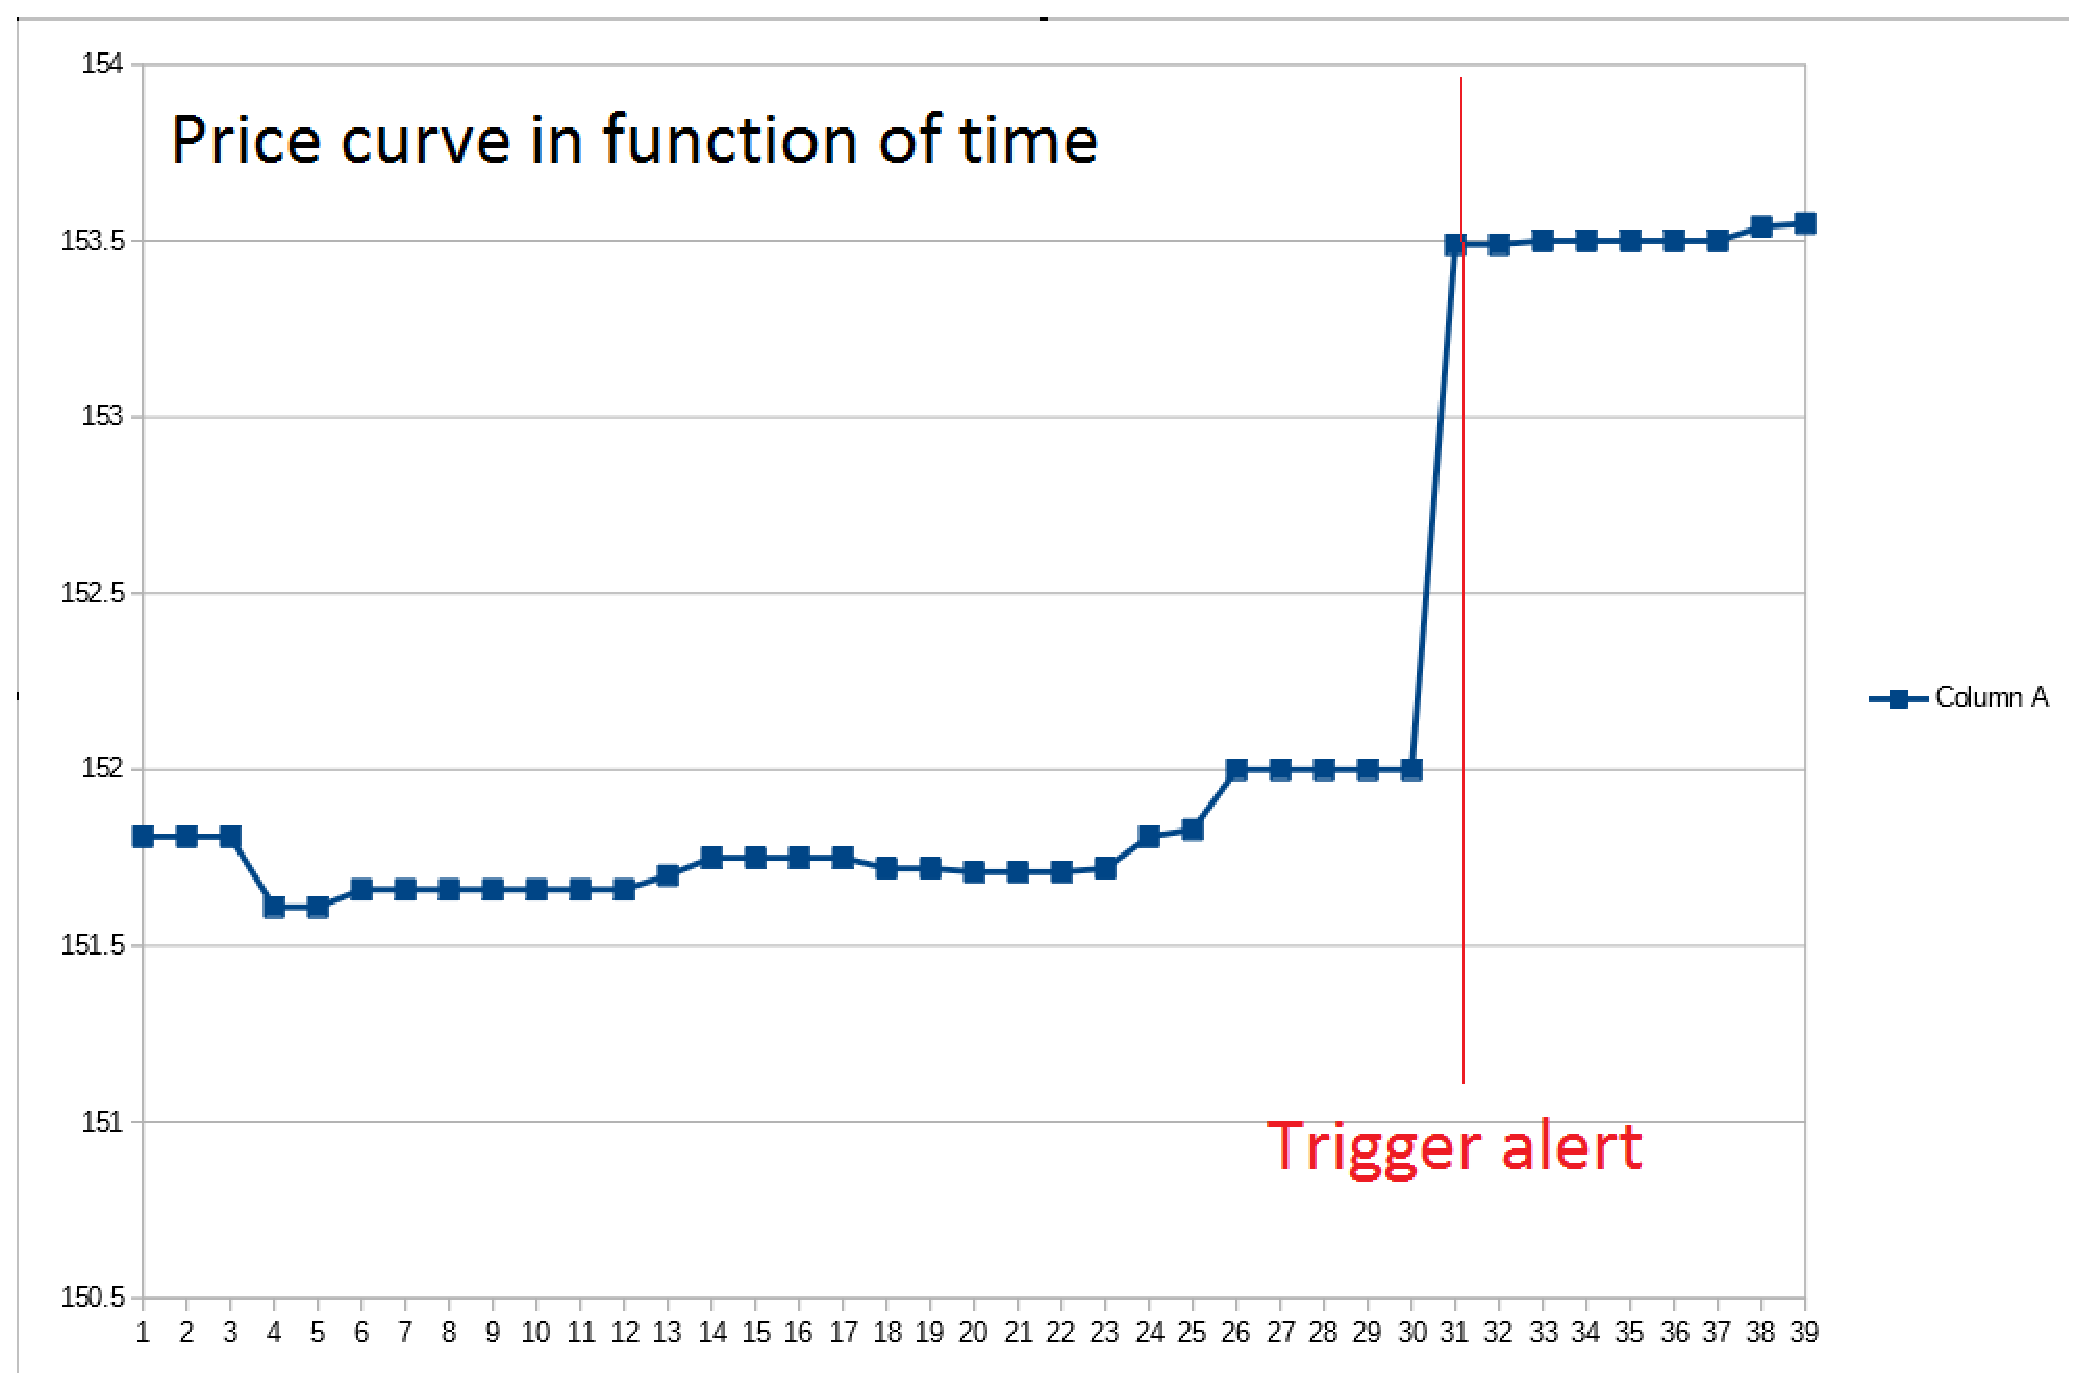
\includegraphics[scale=0.3]{data}
\caption{Abnormal Trade Data}
\label{fig:data}
\end{figure}

\paragraph{Example of data} In figure ~\ref{fig:data}, we see a real Trade data. The vertical axe is the price, the horizontal axe does not exist, but can be viewed as time. At the vertical red line has occurred a abnormal price movement. We would like to write a algorithm to catch that high increase of price and printout a warning text, saying something abnormal happened at that moment and explaining the reason.

\paragraph{To implement}
The candidate has to fill the function \lstinline{AbnormalTrade::process} take a real value in argument, it supposed to be a trading price at the current moment. Candidate can be free to implement this class \lstinline{AbnormalTrade} as far as it inherit from \lstinline{AnalyticsAPI}.

\paragraph{Objective}
\begin{itemize}
	\item An csv example of Trade data is provided. Candidate firstly has to implement the function AbnormalTrade::process that discover when the Trade Price move abnormally, in that case, print to console a warning message.
	\item Candidate is then supposed to create a various different data, of different variation and different size (up to 1M points) to test the program. Can use Excel/R/Matlab or any tool to generate the data. 
	\item At the end, write a short report (2 pages max) with some screenshots commenting how good is the algorithm, in term of accuracy, interm of performance. What was the challenges.
\end{itemize}


\end{document}
